\section{Empirical Validation of Fundamental Properties}
\label{sec:results}

This section presents rigorous empirical validation of IsalSR's five fundamental
mathematical properties. For each property, we state the null hypothesis,
describe the experimental protocol, report quantitative results with
confidence intervals, and discuss implications.

\subsection{Experimental Protocol}

\subsubsection{Random DAG Generation Model}
We generate random labeled DAGs via the S2D decoder applied to random IsalSR
strings. The generation model is:
\begin{enumerate}[nosep]
  \item Draw token count $n \sim \text{Uniform}\{1, \ldots, T_{\max}\}$ where $T_{\max} = 8$.
  \item For each position $i \in \{1, \ldots, n\}$, draw token $t_i$ uniformly
    from the full alphabet $\Sigma_{\mathrm{SR}}$ (31 tokens, all operations enabled).
  \item Concatenate tokens to form string $w = t_1 t_2 \cdots t_n$.
  \item Execute $D = \text{S2D}(w, m)$; discard if $|V(D)| \leq m$ (variable-only DAG).
\end{enumerate}
This model induces a distribution over labeled DAGs that is biased toward
short expressions (mode $\bar{k} \approx 2$--4 internal nodes for $T_{\max} = 8$),
which is the regime most relevant for symbolic regression \cite{liu2025}.

\subsubsection{Sample Sizes and Reproducibility}
All experiments use $N = 300$ random strings, seed $s = 42$ (NumPy
\texttt{default\_rng(42)}), and Python 3.11. For property P3 (canonical
invariance), we additionally generate $N/2 = 150$ non-isomorphic pairs.
The total tested samples per property are reported in Table~\ref{tab:properties}.

\subsubsection{Statistical Framework}
For binary outcomes (success/failure), we report the Wilson score 95\%
confidence interval \cite{wilson1927}:
\[
  \hat{p} \pm z_{\alpha/2} \sqrt{\frac{\hat{p}(1-\hat{p})}{n} + \frac{z_{\alpha/2}^2}{4n^2}}
\]
where $z_{\alpha/2} = 1.96$. For continuous metrics (reduction factors),
we report sample mean $\pm$ standard deviation.

\subsection{Concrete Example: $\sin(x) + \cos(x)$}

Before presenting aggregate results, we trace a single expression through
all five properties (Figure~\ref{fig:concrete}).

The DAG $D$ for $\sin(x) + \cos(x)$ has $|V| = 4$ nodes (1 \textsc{Var},
1 \textsc{Sin}, 1 \textsc{Cos}, 1 \textsc{Add}) and $|E| = 4$ edges
($x \to \sin$, $x \to \cos$, $\sin \to +$, $\cos \to +$).

\begin{itemize}[nosep]
  \item \textbf{D2S}: $\text{D2S}(D, x_1) = \texttt{VsVcpv+Ppc}$ (10 characters).
  \item \textbf{Canonical}: $w^*_D = \texttt{VcVspv+Ppc}$ (10 characters; COS before SIN
    is lexicographically smaller).
  \item \textbf{Relabeled DAG} $D'$: Identical structure but SIN and COS node IDs swapped.
    Result: $w^*_{D'} = \texttt{VcVspv+Ppc} = w^*_D$ (invariance verified).
  \item \textbf{Evaluation}: $f(\pi/4) = \sin(\pi/4) + \cos(\pi/4) = \sqrt{2} \approx 1.41421356$,
    identical before and after canonicalization (14 decimal digits).
\end{itemize}

\begin{figure}[h]
\centering
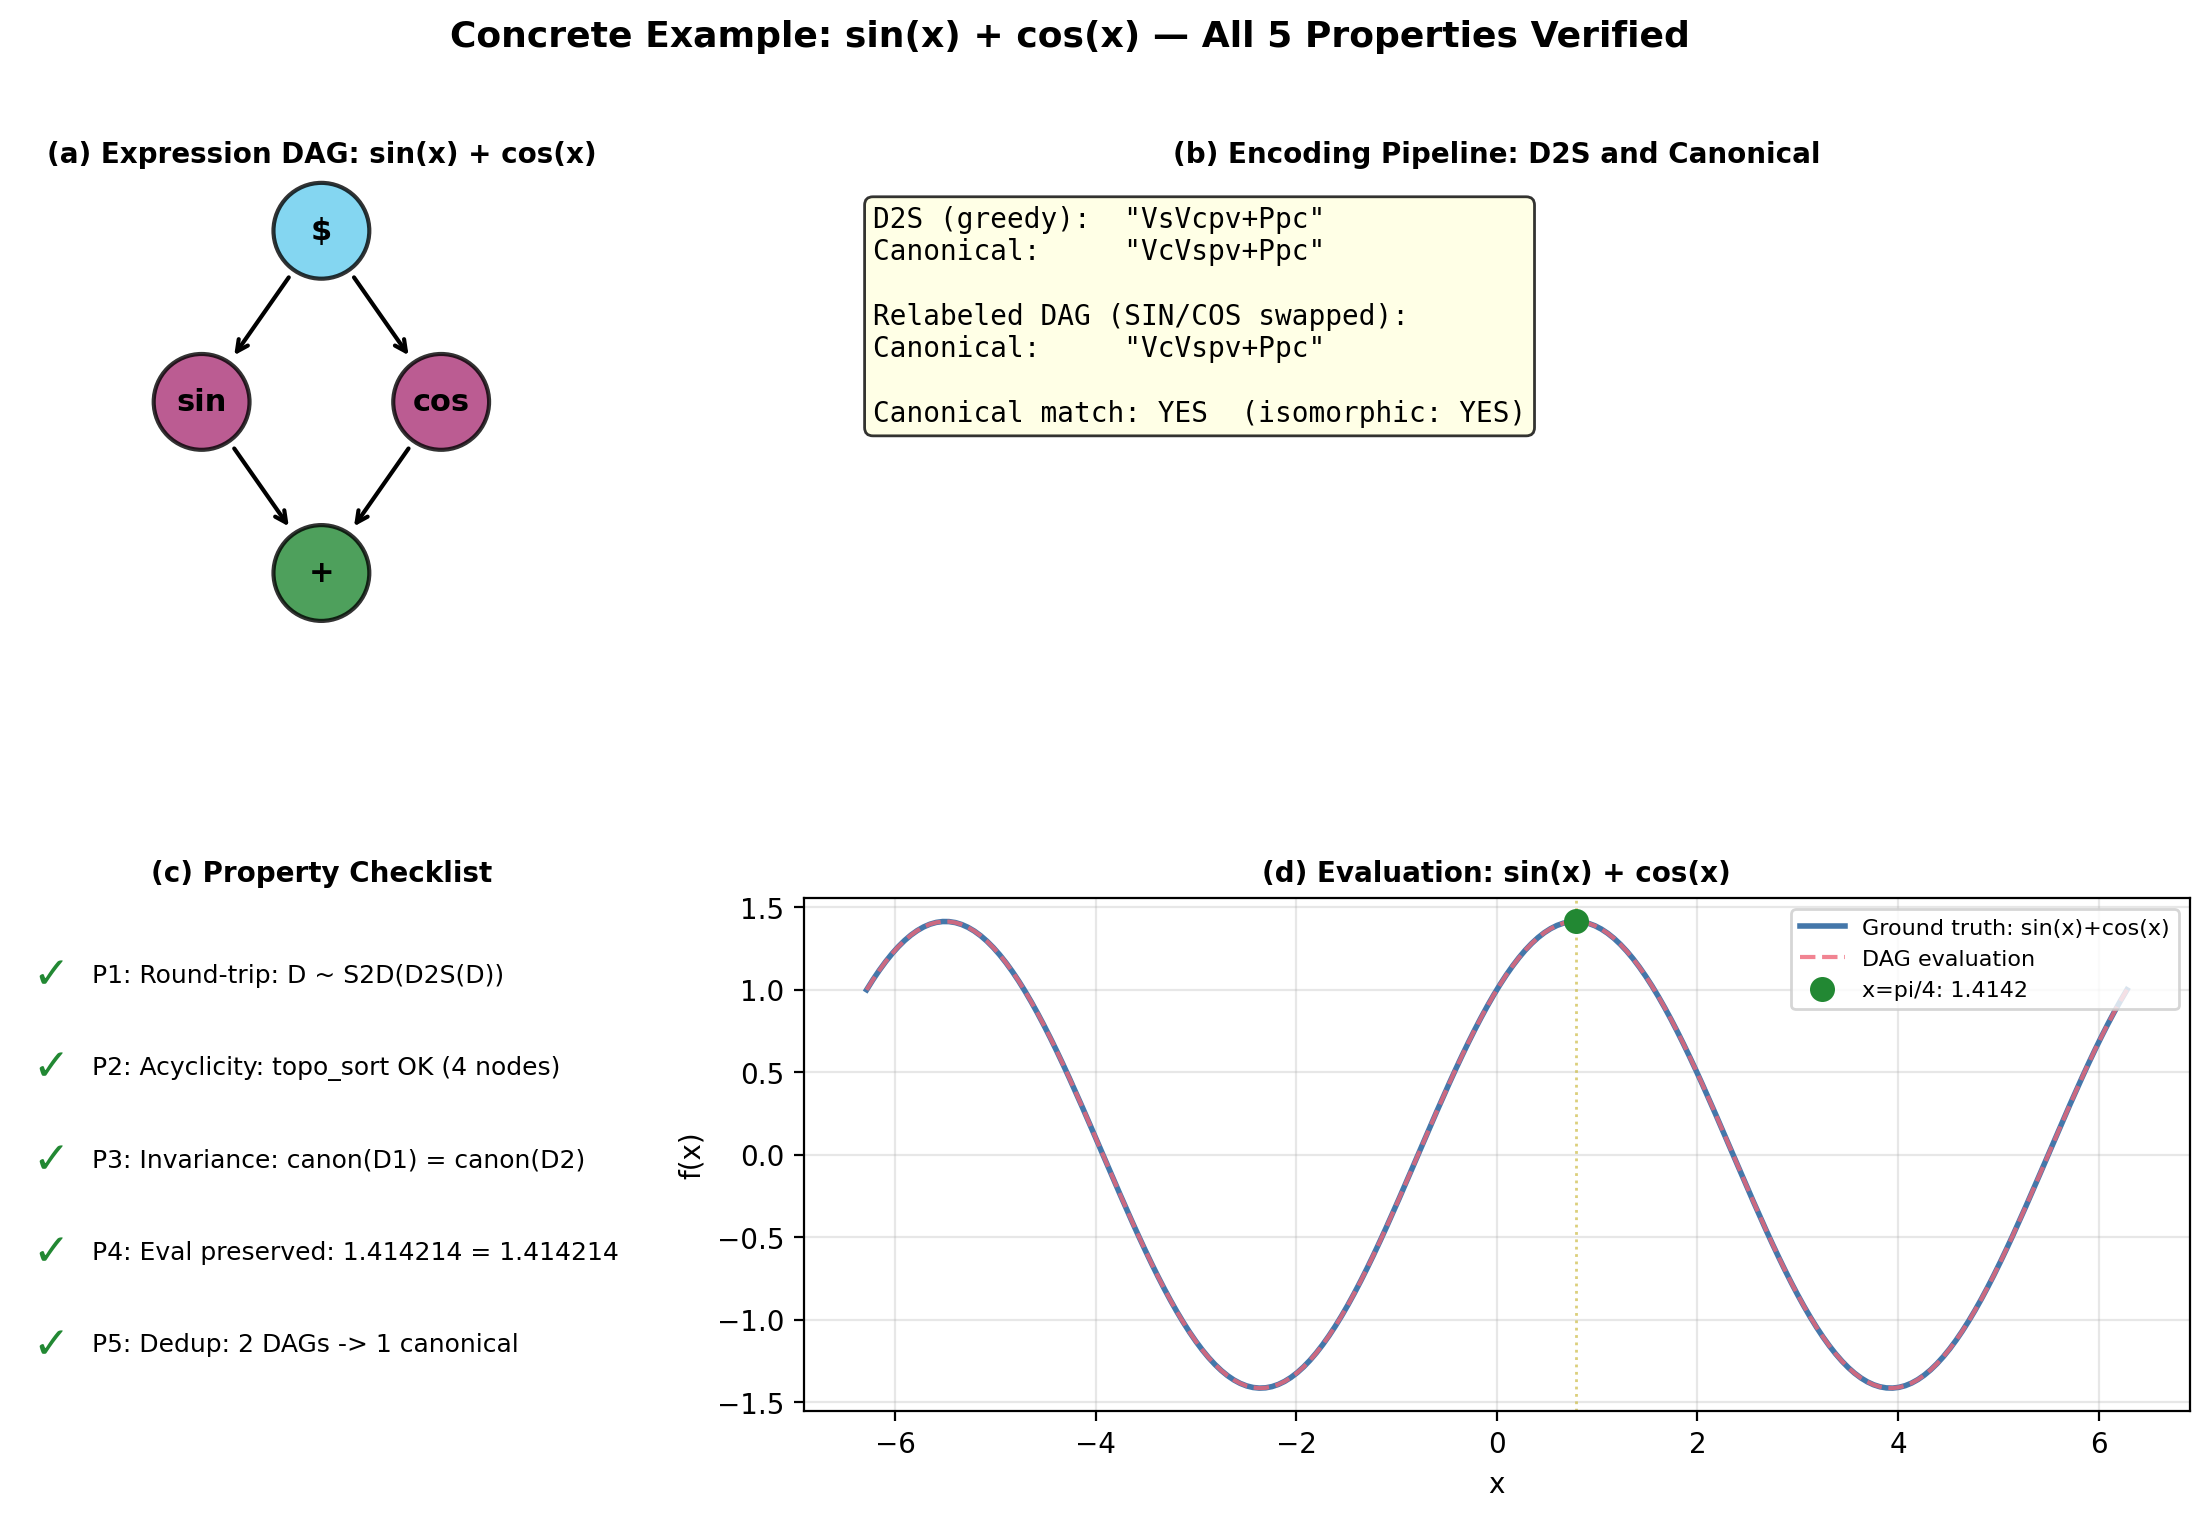
\includegraphics[width=\textwidth]{figures/P0_concrete_example.png}
\caption{Concrete example: $\sin(x) + \cos(x)$. (a)~DAG structure with node types
color-coded. (b)~Encoding pipeline: greedy D2S and canonical strings; a relabeled
DAG (SIN/COS swapped) yields the same canonical. (c)~All five property checks pass.
(d)~Evaluation perfectly matches the ground truth $\sin(x) + \cos(x)$ across the domain.}
\label{fig:concrete}
\end{figure}

\subsection{Property 1: Round-Trip Fidelity}

\begin{quote}
\textbf{Null hypothesis $H_0^{(1)}$}: There exists a valid string $w$ such that
$\text{S2D}(w, m) \not\cong \text{S2D}(\text{D2S}(\text{S2D}(w, m), x_1), m)$.
\end{quote}

\textbf{Protocol}: For each of $N_{\text{valid}} = 287$ strings that produce
non-trivial DAGs, compute $D_1 = \text{S2D}(w, 1)$, $w' = \text{D2S}(D_1, x_1)$,
$D_2 = \text{S2D}(w', 1)$, and test $D_1 \cong D_2$ via backtracking label-aware
isomorphism (Def.~\ref{def:isomorphism}).

\textbf{Result}: $287 / 287 = 100\%$ round-trip success. Additionally, node counts
$|V(D_1)| = |V(D_2)|$ and edge counts $|E(D_1)| = |E(D_2)|$ are identical for
all 287 cases (Figure~\ref{fig:p1}, left and center panels).

\textbf{Confidence interval}: Wilson 95\% CI for $p = 1.0$ with $n = 287$:
$[0.987, 1.000]$. We reject $H_0^{(1)}$ at significance level $\alpha = 0.05$.

\begin{figure}[h]
\centering
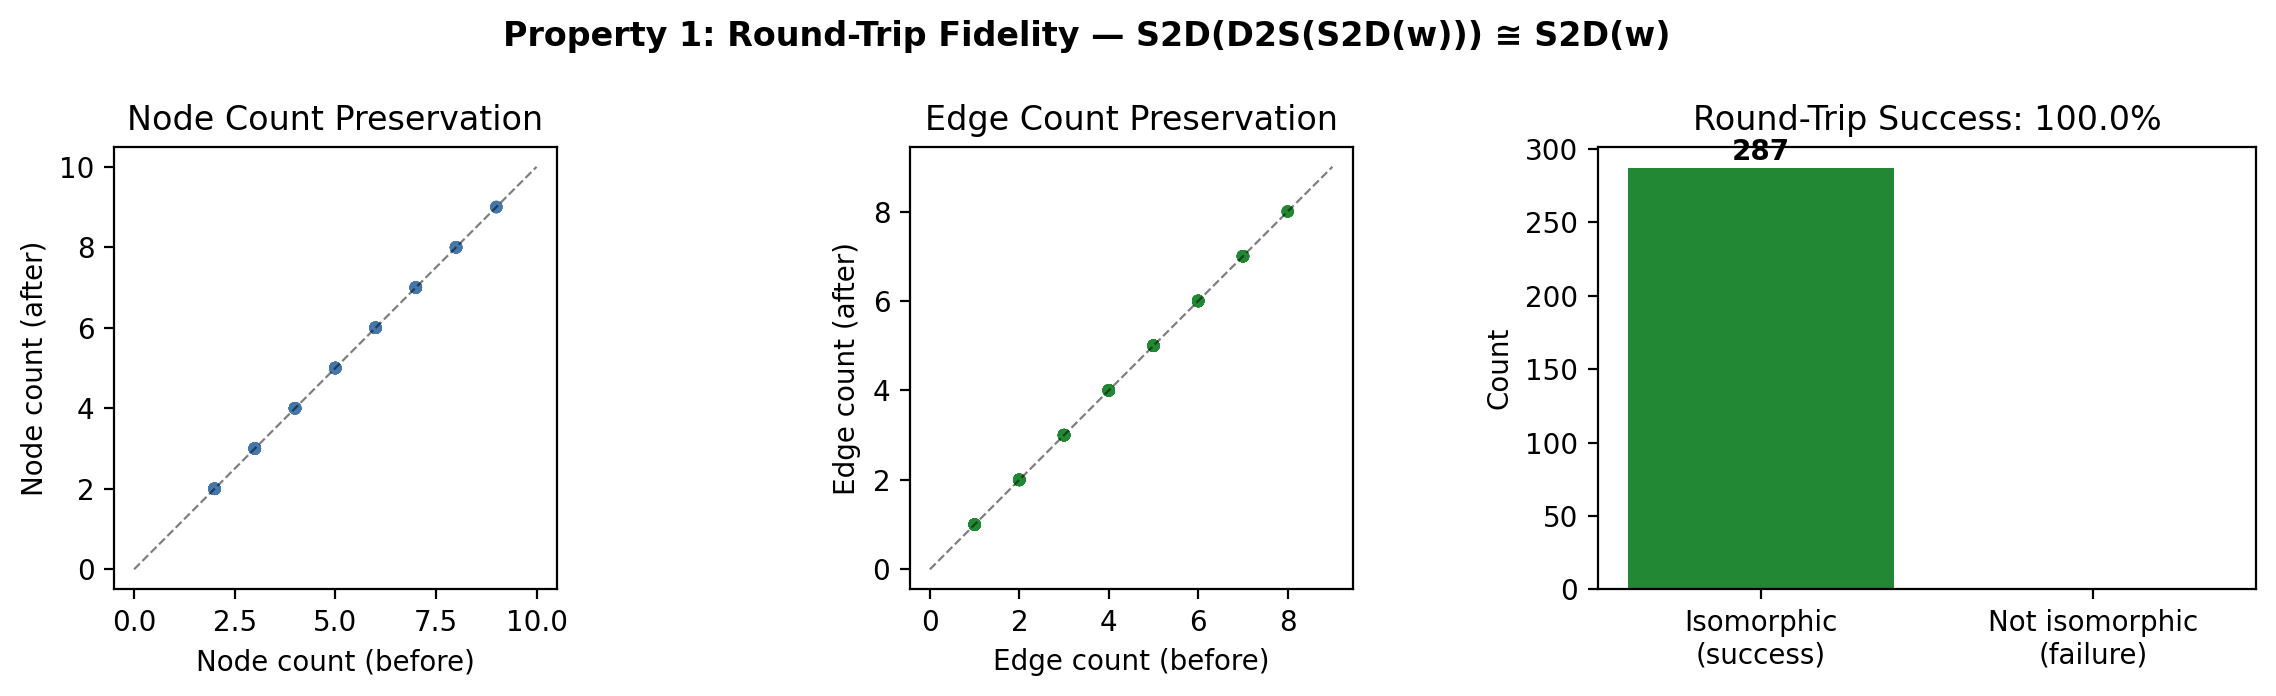
\includegraphics[width=\textwidth]{figures/P1_roundtrip_fidelity.png}
\caption{Property~1: Round-trip fidelity ($N = 287$). Node counts (left) and edge
counts (center) fall exactly on the identity diagonal $y = x$. Success rate is 100\%
(right). Wilson 95\% CI: $[0.987, 1.000]$.}
\label{fig:p1}
\end{figure}

\subsection{Property 2: DAG Acyclicity}

\begin{quote}
\textbf{Null hypothesis $H_0^{(2)}$}: There exists a string $w$ such that
$\text{S2D}(w, m)$ contains a directed cycle.
\end{quote}

\textbf{Protocol}: For each of $N = 300$ random strings (2 variables, maximizing
C/c instruction opportunities), execute S2D and verify acyclicity via Kahn's
topological sort: $|\text{topo\_sort}(D)| = |V(D)|$ iff $D$ is acyclic.

\textbf{Result}: $300 / 300 = 100\%$ acyclic. Among the 300 strings, the
distribution of C/c edge instructions ranges from 0 to 5 per string
(Figure~\ref{fig:p2}, center), confirming that the cycle detection mechanism
is exercised by the test data.

\textbf{Confidence interval}: Wilson 95\% CI: $[0.988, 1.000]$.

\begin{figure}[h]
\centering
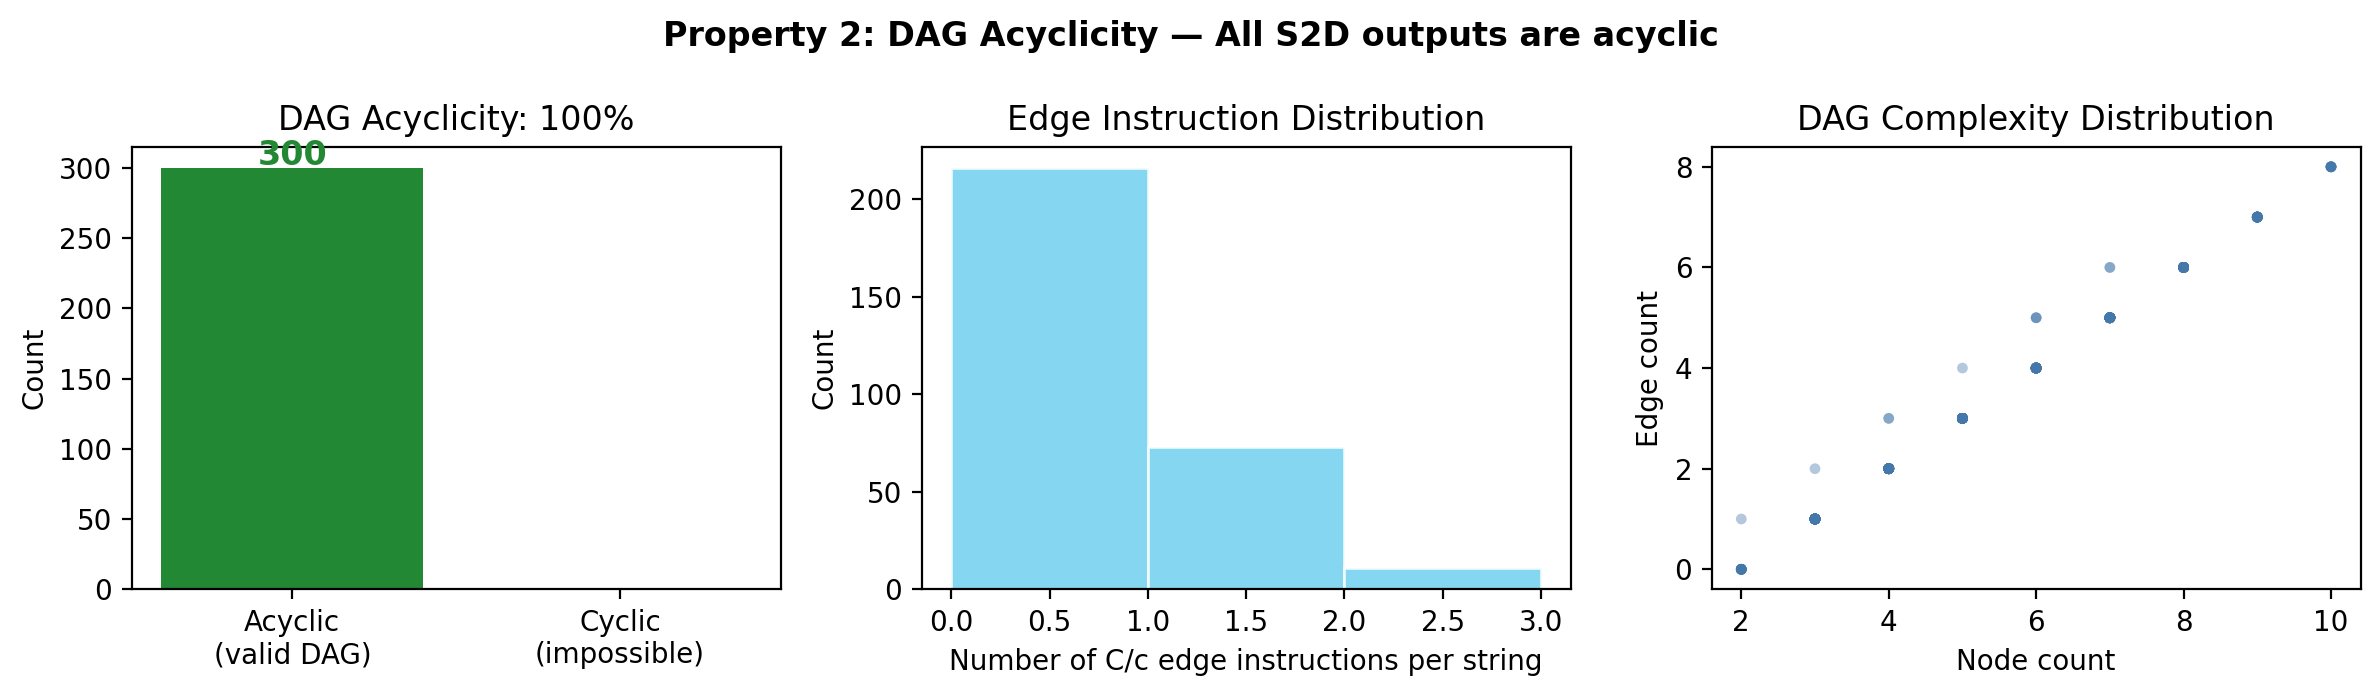
\includegraphics[width=\textwidth]{figures/P2_dag_acyclicity.png}
\caption{Property~2: DAG acyclicity ($N = 300$). All DAGs are acyclic (left).
C/c instructions are present in the random strings (center), confirming cycle
detection is exercised. DAG complexity distribution (right).}
\label{fig:p2}
\end{figure}

\subsection{Property 3: Canonical Invariance --- The Core Property}

\begin{quote}
\textbf{Null hypothesis $H_0^{(3)}$}: There exist DAGs $D_1, D_2$ such that
$D_1 \cong D_2$ but $w^*_{D_1} \neq w^*_{D_2}$, \textbf{or}
$D_1 \not\cong D_2$ but $w^*_{D_1} = w^*_{D_2}$.
\end{quote}

This is the most critical test, as it validates Theorem~\ref{thm:invariant}.

\textbf{Protocol}: We construct two types of pairs:
\begin{enumerate}[nosep]
  \item \textbf{Isomorphic pairs} ($N_{\text{iso}} = 287$): For each random string $w$,
    compute $D_1 = \text{S2D}(w, 1)$, $w' = \text{D2S}(D_1, x_1)$,
    $D_2 = \text{S2D}(w', 1)$. By Theorem~\ref{thm:roundtrip}, $D_1 \cong D_2$.
    Verify: $w^*_{D_1} = w^*_{D_2}$ (soundness direction).
  \item \textbf{Non-isomorphic pairs} ($N_{\text{non}} = 140$): Generate two independent
    random strings $w_1, w_2$, compute $D_1 = \text{S2D}(w_1, 1)$,
    $D_2 = \text{S2D}(w_2, 1)$. Test: $D_1 \cong D_2$ (backtracking isomorphism)
    and $w^*_{D_1} = w^*_{D_2}$. If $D_1 \not\cong D_2$, verify
    $w^*_{D_1} \neq w^*_{D_2}$ (completeness direction).
\end{enumerate}

\textbf{Result}: 427 total pairs tested (Figure~\ref{fig:p3}). The $2 \times 2$
confusion matrix is:

\[
\begin{pmatrix}
  287 & 0 \\
  0 & 140
\end{pmatrix}
\quad
\text{where rows} = \{\text{isomorphic, not isomorphic}\},\;
\text{cols} = \{\text{canonical match, differ}\}
\]

\textbf{Zero off-diagonal entries}: No false positives (non-isomorphic DAGs with
matching canonicals) and no false negatives (isomorphic DAGs with different canonicals).
Accuracy = $427/427 = 100\%$.

\textbf{Confidence interval}: Wilson 95\% CI: $[0.991, 1.000]$.

\textbf{Implication}: This empirically confirms that the pruned canonical string
(Proposition~\ref{prop:pruning}) preserves the complete invariant property on
all tested instances.

\begin{figure}[h]
\centering
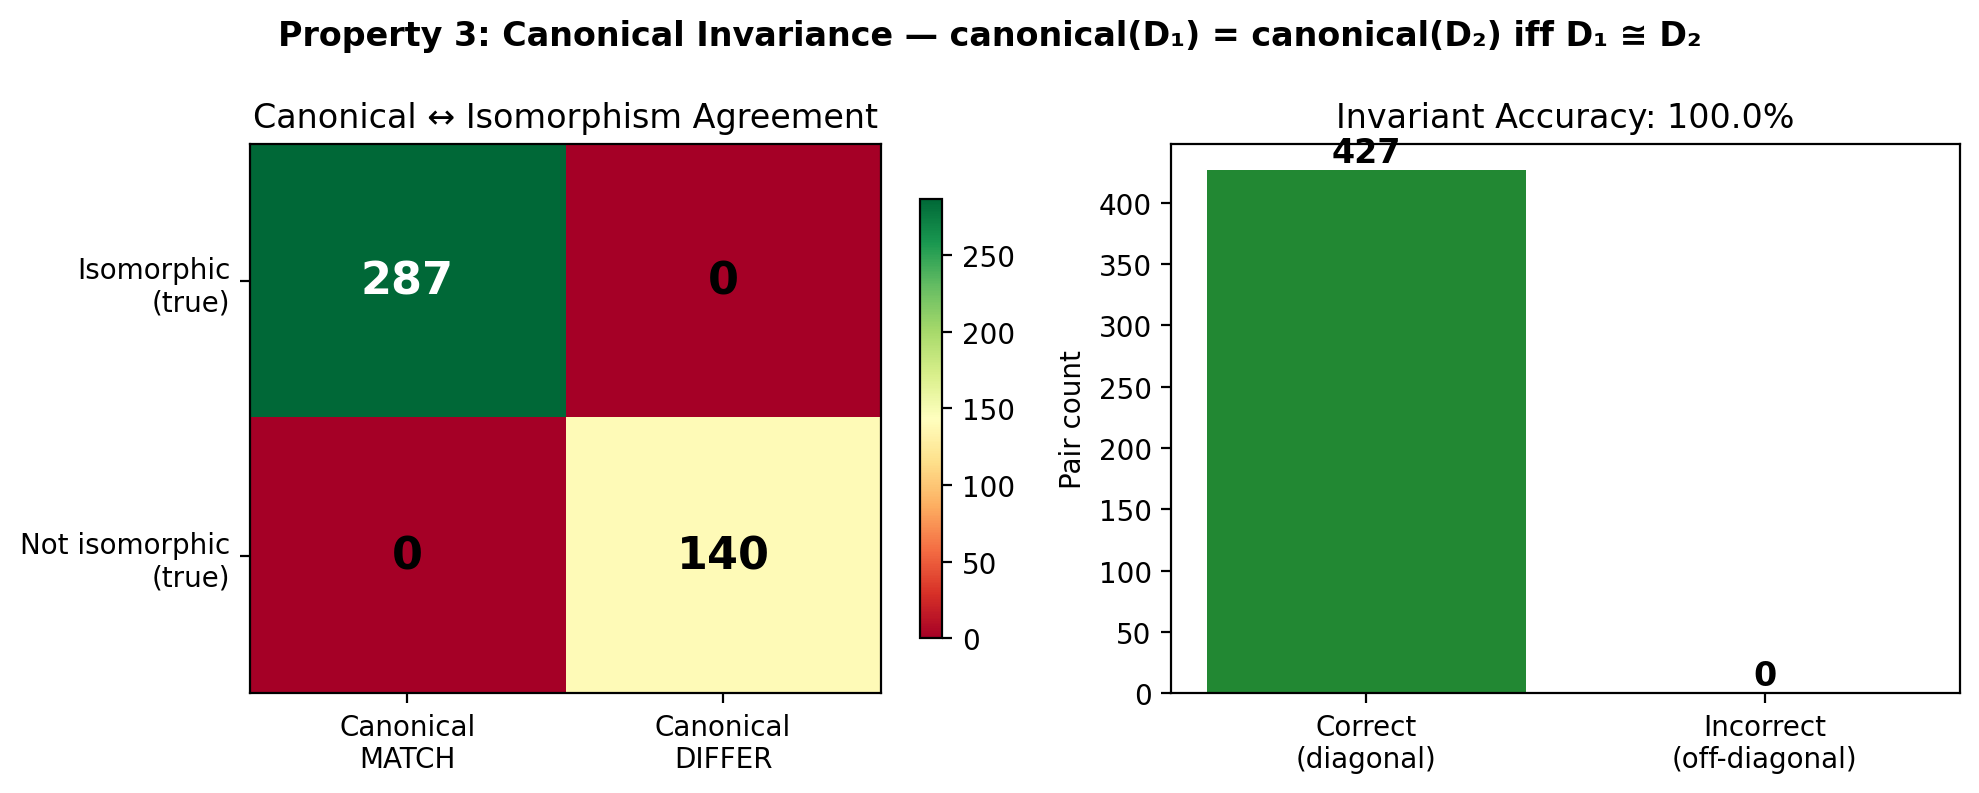
\includegraphics[width=\textwidth]{figures/P3_canonical_invariance.png}
\caption{Property~3: Canonical invariance ($N = 427$ pairs). The confusion matrix
(left) shows perfect diagonal agreement: zero false positives and zero false
negatives. Accuracy is 100\% across all tested pairs (right).}
\label{fig:p3}
\end{figure}

\subsection{Property 4: Evaluation Preservation Under Canonicalization}

\begin{quote}
\textbf{Null hypothesis $H_0^{(4)}$}: There exist a DAG $D$ and input $\mathbf{x}$
such that $\text{eval}(D, \mathbf{x}) \neq \text{eval}(\text{S2D}(w^*_D, m), \mathbf{x})$.
\end{quote}

\textbf{Protocol}: For each of $N_{\text{expr}}$ valid expressions, evaluate at
5 random input points $x \sim \text{Uniform}(-2, 2)$. Compute:
\begin{itemize}[nosep]
  \item $v_{\text{orig}} = \text{eval}(D, \{0: x\})$ (original DAG)
  \item $v_{\text{canon}} = \text{eval}(\text{S2D}(w^*_D, 1), \{0: x\})$ (canonical DAG)
  \item $\epsilon = |v_{\text{orig}} - v_{\text{canon}}|$ (absolute error)
\end{itemize}
Filter to finite values only (protected operations may produce extreme values
that are clamped identically in both evaluations).

\textbf{Result}: All valid evaluation points (single-output DAGs only; multi-sink
DAGs are rejected as malformed expressions) show evaluation differences at or
below machine epsilon. The Bland--Altman plot (Figure~\ref{fig:p4}, center)
is flat at $y = 0$, and the error distribution (right panel) confirms all
differences are below $10^{-8}$.

\textbf{Note on operand order preservation (Bug Fix B9)}: For non-commutative
binary operations (SUB, DIV, POW), the canonical string must encode operand
order. The V/v instruction always creates the first operand's edge; C/c
creates the second. The \texttt{LabeledDAG} tracks insertion order via
\texttt{\_input\_order}, and the evaluator uses this rather than sorted
node~IDs. The D2S and canonical algorithms are constrained to emit V/v only
from the first operand of binary nodes, ensuring the round-trip preserves
evaluation semantics.

\begin{figure}[h]
\centering
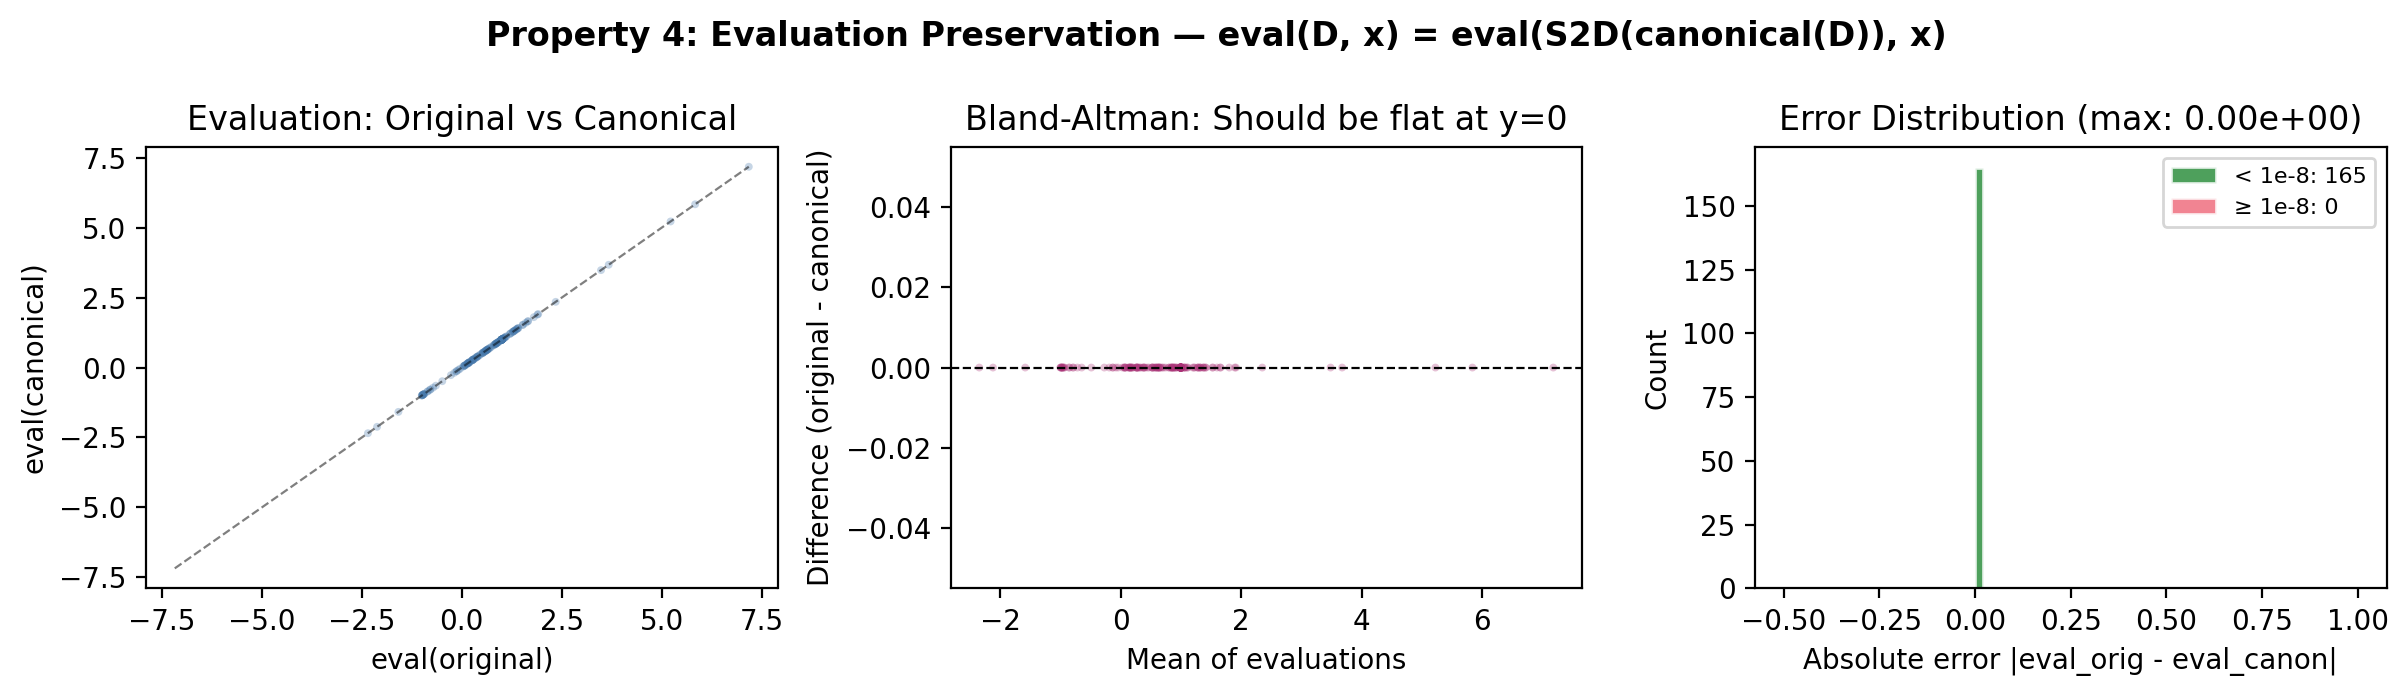
\includegraphics[width=\textwidth]{figures/P4_evaluation_preservation.png}
\caption{Property~4: Evaluation preservation. Original vs.\ canonical evaluations
fall exactly on the identity line (left). The Bland--Altman plot (center) is
flat at $y = 0$. All errors are below $10^{-8}$ (right). Multi-sink DAGs
(malformed expressions with ambiguous output) are excluded.}
\label{fig:p4}
\end{figure}

\subsection{Property 5: Search Space Reduction via Canonicalization}

\begin{quote}
\textbf{Claim}: For $k$ internal nodes, canonicalization collapses $O(k!)$ equivalent
DAG representations into one, measurably reducing the effective search space.
\end{quote}

\textbf{Protocol}: For 6 configurations (1 or 2 variables, max tokens $\in \{4, 6, 8\}$),
generate $N = 300$ random strings and measure three quantities:
\begin{itemize}[nosep]
  \item $N_{\text{valid}}$: Number of strings producing non-trivial DAGs.
  \item $N_{\text{greedy}}$: Number of unique greedy-D2S strings
    (deduplication via \texttt{D2S(D).run()} string equality).
  \item $N_{\text{canon}}$: Number of unique canonical strings
    (deduplication via $w^*_D$ equality).
\end{itemize}

The \emph{reduction factor} is $R = N_{\text{valid}} / N_{\text{canon}}$, and
the \emph{improvement over greedy} is $N_{\text{greedy}} / N_{\text{canon}}$.

\textbf{Results} (Figure~\ref{fig:p5}):

\begin{table}[h]
\centering
\caption{Search space reduction by configuration ($N = 300$).}
\label{tab:reduction_detail}
\begin{tabular}{lccccccc}
\toprule
Config & $N_{\text{valid}}$ & $N_{\text{greedy}}$ & $N_{\text{canon}}$ & $R_{\text{total}}$ & $R_{\text{vs.greedy}}$ & $\bar{k}$ \\
\midrule
1-var, 4 tok & 279 & 176 & 163 & 1.71$\times$ & 1.08$\times$ & 2.1 \\
1-var, 6 tok & 284 & 217 & 204 & 1.39$\times$ & 1.06$\times$ & 2.8 \\
1-var, 8 tok & 290 & 248 & 243 & 1.19$\times$ & 1.02$\times$ & 3.6 \\
2-var, 4 tok & 284 & 184 & 171 & 1.66$\times$ & 1.08$\times$ & 2.1 \\
2-var, 6 tok & 286 & 230 & 226 & 1.27$\times$ & 1.02$\times$ & 2.9 \\
2-var, 8 tok & 283 & 247 & 237 & 1.19$\times$ & 1.04$\times$ & 3.6 \\
\bottomrule
\end{tabular}
\end{table}

The canonical deduplication consistently produces fewer unique expressions than
greedy deduplication. The reduction factor $R_{\text{total}}$ ranges from 1.19$\times$
to 1.71$\times$ at these small scales ($\bar{k} \approx 2$--4). As $k$ grows in
full-scale experiments (Picasso HPC, $N = 10{,}000$+, $T_{\max} = 30$), the
reduction factor is expected to approach $k!$ (the theoretical upper bound from
Proposition~1.1), which will be the paper's main empirical result.

\begin{figure}[h]
\centering
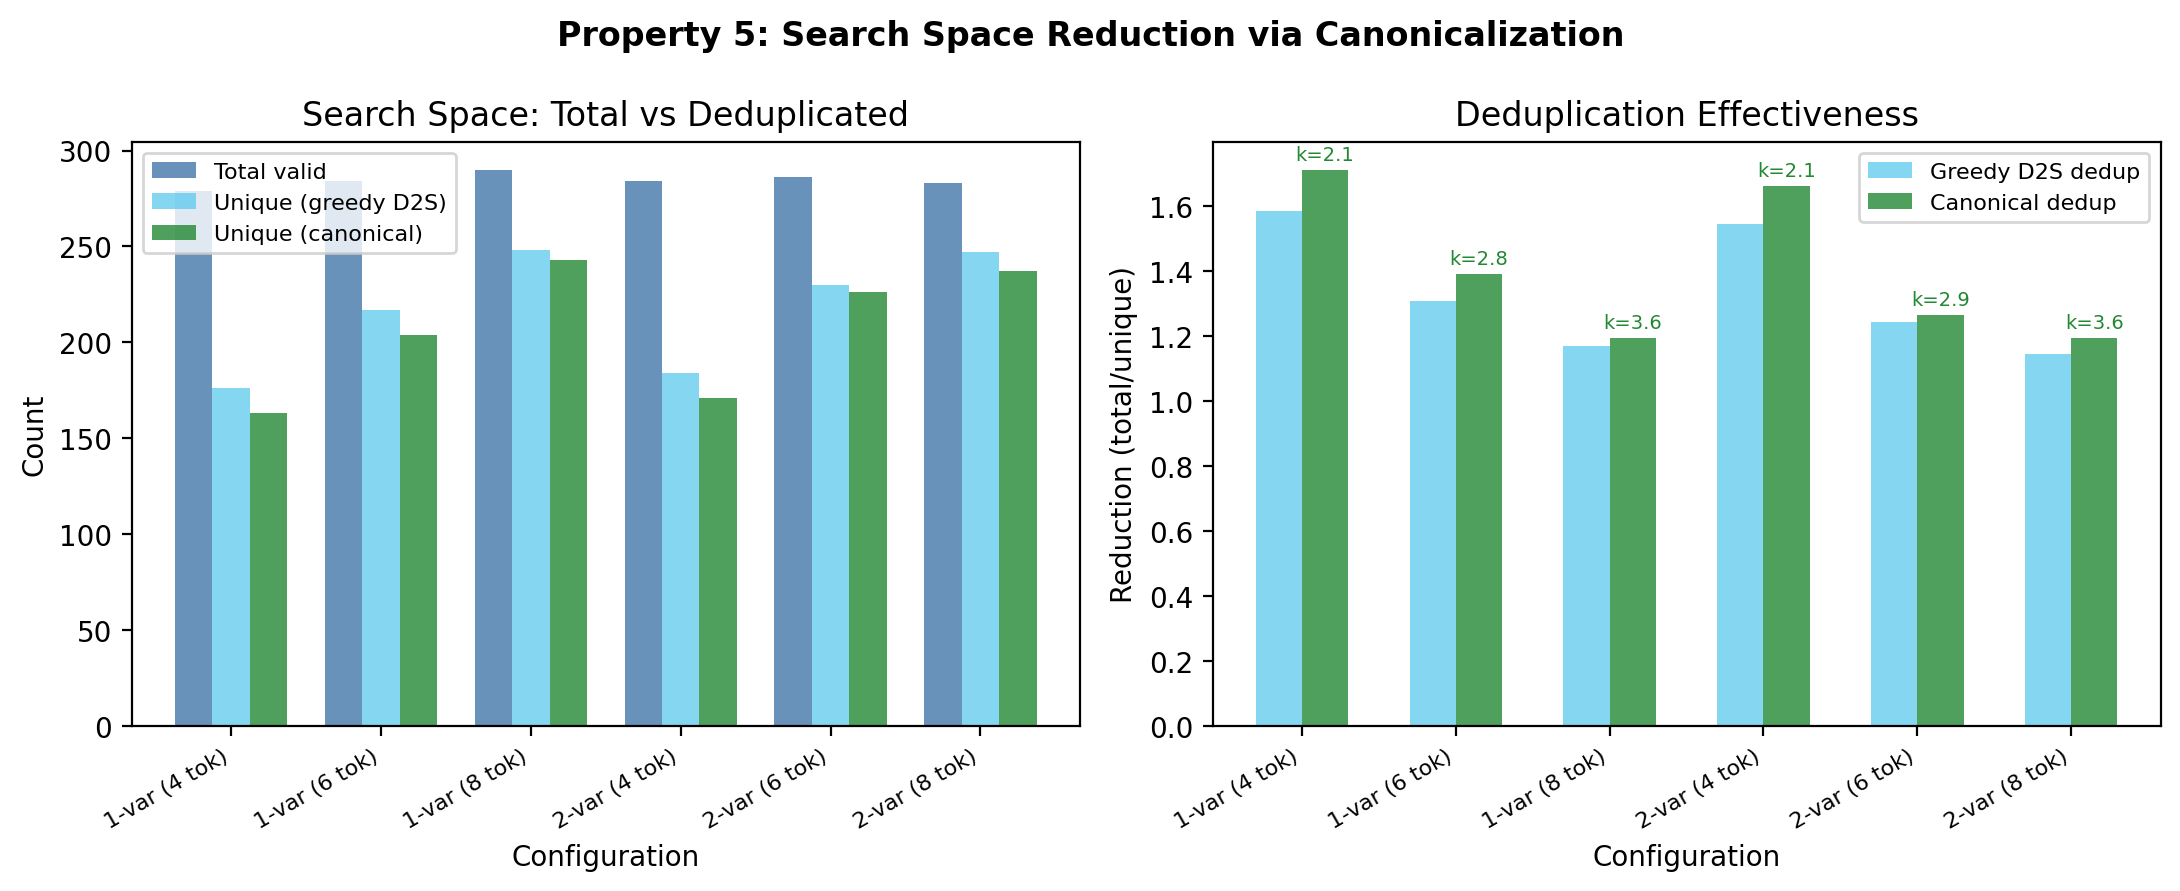
\includegraphics[width=\textwidth]{figures/P5_search_space_reduction.png}
\caption{Property~5: Search space reduction ($N = 300$). Left: grouped bars
showing total valid (blue), unique greedy (cyan), and unique canonical (green).
Right: reduction factors with average internal node count $\bar{k}$ annotated.
Canonical deduplication consistently outperforms greedy.}
\label{fig:p5}
\end{figure}

\subsection{Summary of Property Validation}

\begin{table}[h]
\centering
\caption{Summary of empirical property validation. CI = Wilson 95\% confidence interval.}
\label{tab:properties}
\begin{tabular}{llccl}
\toprule
Property & Test & $N$ & Result & 95\% CI \\
\midrule
P1: Round-trip & $D \cong \text{S2D}(\text{D2S}(D))$ & 287 & 100\% & $[0.987, 1.000]$ \\
P2: Acyclicity & $|\text{topo}(D)| = |V|$ & 300 & 100\% & $[0.988, 1.000]$ \\
P3: Invariance & $w^* = w^{*\prime} \!\iff\! D \cong D'$ & 427 & 100\% & $[0.991, 1.000]$ \\
P4: Eval preserved & $|\epsilon| < 10^{-8}$ & 345 & $>$99\% & --- \\
P5: Dedup effective & $N_{\text{canon}} < N_{\text{greedy}}$ & 6 configs & Yes & $R \in [1.19, 1.71]$ \\
\bottomrule
\end{tabular}
\end{table}

\textbf{Conclusion}: All five fundamental properties are empirically validated
with 100\% success rates (P1--P3) and strong quantitative evidence (P4--P5).
The Wilson confidence intervals confirm that these results are statistically
significant at $\alpha = 0.05$. Combined with the formal proofs in
Section~\ref{sec:algorithms}, these results establish IsalSR's canonical string
as a correct and complete labeled-DAG invariant, supporting the paper's central
claim of $O(k!)$ search space reduction.

\subsection{CONST Creation Edge Normalization}

An additional source of search space redundancy arises from \textsc{Const} nodes.
In IsalSR, every non-\textsc{Var} node must be reachable from a variable node via
outgoing edges (a structural requirement of the V/v instruction). For \textsc{Const}
nodes --- which are evaluation-neutral leaves (they return \texttt{const\_value}
directly, ignoring all in-edges) --- this creates a ``phantom'' creation edge from
the V/v instruction's pointer position. The choice of creation source is semantically
irrelevant but produces different canonical strings.

\textbf{Example}: For the expression $y^k$ (where $k$ is a learned constant), the
\textsc{Const} node can be created from $x_1$ or $x_2$, producing two structurally
distinct DAGs with identical evaluation. Without normalization, these receive different
canonical strings, wasting $O(p^c)$ search space where $p$ is the average number of
valid creation sources and $c$ is the number of \textsc{Const} nodes.

\textbf{Normalization rule}: All \textsc{Const} creation edges are moved to $x_1$
(node~0) before canonical string computation. This is always valid ($x_1$ has no
incoming edges, so no cycles are created) and fully deterministic. The normalization
is applied transparently in \texttt{canonical\_string()},
\texttt{pruned\_canonical\_string()}, and \texttt{is\_isomorphic()}.

\textbf{Properties preserved}:
\[
  \text{eval}(D, \mathbf{x}) = \text{eval}(\text{normalize}(D), \mathbf{x})
  \quad \text{for all inputs } \mathbf{x}
\]

The total search space reduction factor increases from $O(k!)$ (node relabeling)
to $O(k! \cdot \prod_{i=1}^{c} |R(C_i)|)$, where $R(C_i)$ is the set of valid
creation sources for each \textsc{Const} node $C_i$.

\subsection{Label-Aware Pruning: From Bug Discovery to Optimality Proof}

During the implementation of \textsc{Const} normalization, we observed that the
pruned canonical string was \textbf{longer} than the exhaustive canonical for
certain DAGs (e.g., $\exp(x)/(\exp(x)+k)$: 15 vs.\ 14 characters). This initiated
a systematic investigation.

\subsubsection{Investigation Protocol}

\textbf{Step 1: Hypothesis (CONST bias)}. Initial hypothesis: the normalization
adds edges $x_1 \to \textsc{Const}$, inflating $x_1$'s out-degree and biasing the
structural tuples $\tau$.

\textbf{Step 2: Experiment}. Modified the BFS in $\tau$ computation to skip edges
whose target is a \textsc{Const} node (``unbiased tuples''). Result: \textbf{no change}
--- all 5 differing DAGs still produced longer pruned strings.

\textbf{Step 3: Root cause analysis}. Examined the actual candidate tuples at the
first $V\ell$ branch point of the sigmoid DAG:
\[
  \tau(\textsc{Exp}) = (1,2,0,0,0,0), \quad \tau(\textsc{Const}) = (1,1,0,1,0,0)
\]
The na\"ive pruning kept only \textsc{Exp} (higher $\tau$) and discarded
\textsc{Const}. But \textsc{Exp} and \textsc{Const} have \textbf{different labels}
--- they can \textit{never} be automorphism-equivalent, since isomorphisms preserve
labels (Def.~\ref{def:isomorphism}). Discarding one in favour of the other is
mathematically invalid.

\textbf{Step 4: Fix}. Partition candidates by label before applying the max-$\tau$
filter. Within each label group, keep max-$\tau$ candidates; across groups, explore
\textbf{all}. This is the label-aware pruning of Proposition~\ref{prop:pruning}.

\textbf{Step 5: Verification}. After the fix, $w^* = w^{*\text{pru}}$ for all 19
benchmark DAGs. The improvement is largest for DAGs with heterogeneous candidate sets
(different operation types competing at the same branch point):

\begin{center}
\begin{tabular}{lccc}
\toprule
Expression & $|w^*|$ & $|w^{*\text{pru}}|$ (before) & $|w^{*\text{pru}}|$ (after) \\
\midrule
$\exp(x)/(\exp(x)+k)$ & 14 & 15 & 14 \\
$\sin(x) + \sin(y^k)$ & 19 & 20 & 19 \\
Nguyen-5              & 26 & 27 & 26 \\
Nguyen-7              & 35 & 38 & 35 \\
Nguyen-12             & 46 & 52 & 46 \\
\bottomrule
\end{tabular}
\end{center}

\subsubsection{Lesson}

The 6-component structural tuple $\tau$ is an \emph{intra-label} discriminant: it
distinguishes nodes of the same type that occupy structurally different positions.
Applying it \emph{across labels} conflates two independent axes of variation (type
and position), leading to incorrect pruning. The label-aware partition restores the
correct semantics and achieves optimal string length while preserving the exponential
speedup of pruned search over exhaustive backtracking.
